
\documentclass[a4paper,12pt]{article} 
\usepackage[top = 2.5cm, bottom = 2.5cm, left = 2.5cm, right = 2.5cm]{geometry} 
\usepackage[T1]{fontenc}
\usepackage[utf8]{inputenc}
\usepackage{multirow} 
\usepackage{amsmath}
\usepackage{amssymb}
\usepackage{booktabs} 
\usepackage{graphicx} 
\usepackage{setspace}
\setlength{\parindent}{0in}
\usepackage{float}
\usepackage{tablefootnote}
\usepackage{fancyhdr}
\usepackage[english]{babel}
\usepackage{xcolor}
\usepackage{multirow}
\usepackage{listings}
\usepackage{dcolumn}
\lstset{
  basicstyle=\footnotesize\ttfamily,
  columns=fullflexible,
  frame=single,
  breaklines=true,
  postbreak=\mbox{\textcolor{red}{$\hookrightarrow$}\space},
}
\usepackage{hyperref}
 \hypersetup{
     colorlinks=true,
     linkcolor=black,
     filecolor=black,
     citecolor = black,      
     urlcolor=blue,
     }
\usepackage{csvsimple}
\pagestyle{fancy} 
\fancyhf{} 
\lhead{\footnotesize Economics 714: PS1}
\rhead{\footnotesize Javier Tasso} 
\cfoot{\footnotesize \thepage} 




\begin{document}





\begin{tabular}{p{15.5cm}} 
{\large \bf Economics 714 - Computational Methods in Economics} \\
University of Pennsylvania \\ Fall 2021 \\ \\ 
\hline 
\\
\end{tabular} 

\vspace*{0.3cm} 

\begin{center} 
	{\Large \bf Problem Set 1} 
	\vspace{2mm}
	
        
	{\bf Javier Tasso} 
		
\end{center}  

\vspace{0.4cm}

%%%%%%%%%%%%%%%%%%%%%%%%%%%%%%%%%%%%%%%%%%%%%%%%
%%%%%%%%%%%%%%%%%%%%%%%%%%%%%%%%%%%%%%%%%%%%%%%%



    % Exercise 1    
    
     
    \textbf{Question 1} 
    \medskip

    See \href{https://github.com/javiertasso/econ714_hw1_tasso}{this link}. 

     
    
    % Exercise 2   
    
    \medskip
    \medskip
    \textbf{Question 2} 
    \medskip
    
    Figure (\ref{area_part2}) plots the area we want to calculate and table (\ref{table_ex2}) shows the results using different methods. The code \textit{econ714\_homework1\_question2.m} produces these outputs.  
    
    \begin{figure}[!htbp]
        \centering
       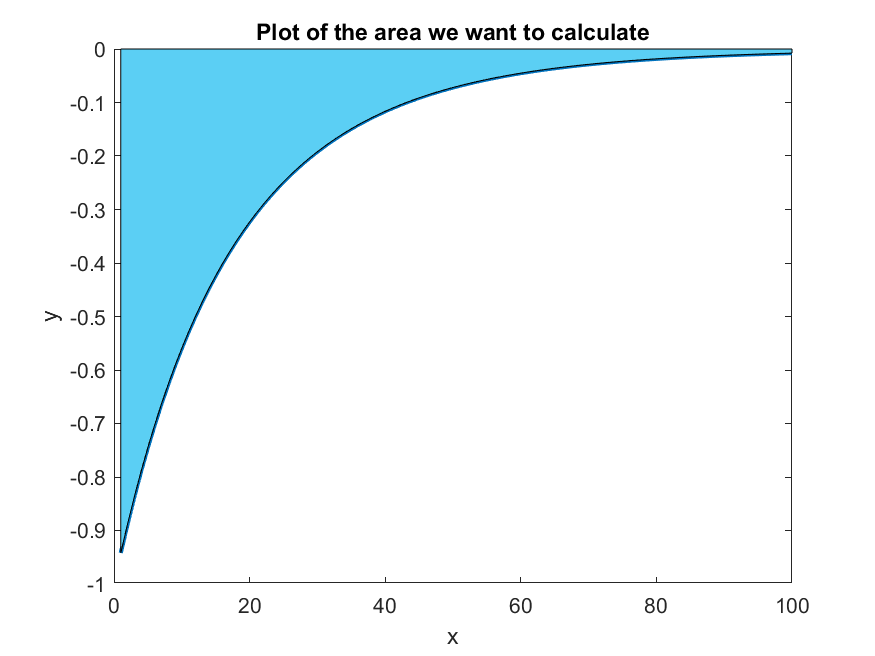
\includegraphics{econ714_homework1_question2_plot.png}
        \caption{Area - Question $2$} 
        \label{area_part2}
    \end{figure}
    
    \begin{table}[!htbp]
        \centering
        \caption[Short Caption for LoT]{Comparison of Different Methods - Question 2}\label{table_ex2}
    \csvautobooktabular{econ714_homework1_question2_output.csv}
    \end{table}
    
 
    
    % Exercise 3   
    
    \medskip
    \medskip
    \textbf{Question 3} 
    \medskip
    
    
    
    
    % Exercise 4  
    
    \medskip
    \medskip
    \textbf{Question 4} 
    \medskip
    
    
    
    % Exercise 5  
    
    \medskip
    \medskip
    \textbf{Question 5} 
    \medskip
    
    
    
  

    

%\hfill

%\pagebreak 

%\pagestyle{empty}

%\section*{Codes}


    %\begin{lstlisting}[language= R]
    
%-


    
    %\end{lstlisting}

    
    
 \end{document}
 